\documentclass[12pt,letterpaper,portrait,onecolumn,titlepage,twoside,final,openright]{book}
\usepackage[utf8x]{inputenc}
\usepackage[T1]{fontenc}			%Para que detecte los acentos
\usepackage[spanish]{babel} 
%\usepackage[none]{hyphenat}		%Libreria para no cortar palabras(no Hipenacion). Usar con Sloppy
%\usepackage{resizebox}
\usepackage{amsmath}
\usepackage{amsthm}
\usepackage{graphicx}
\usepackage{color}
\usepackage{inputenc}
\usepackage{amsfonts}
\usepackage{amssymb}
\usepackage{geometry}
\usepackage{epsfig}
\usepackage{array}
\usepackage{adjustbox}
\usepackage{url}

\usepackage{colortbl} 						% Para el color en la tabla. Junto con color
\usepackage[Lenny]{fncychap}

%\usepackage[bookmarks=true]{hyperref} 		%Pone los marcadores en el pdf. Compilar con: dvi->ps, ps->pdf
\usepackage[hidelinks]{hyperref}			%Ocultar recuadros de vinculos
\usepackage{bookmark}                 		%Pone los marcadores en el pdf. Compilar con: dvi->ps, ps->pdf

%Cambiar color de vinculos
\usepackage{xcolor}

\hypersetup
{
    colorlinks,
    linkcolor={red!50!black},
    citecolor={blue!50!black},
    urlcolor={blue!80!black}
}

\usepackage{listings}	%Insertar programas en C
\usepackage{graphicx} %Utilizar figuras e imagenes
\usepackage{float}
\usepackage{subfig}		%Multiples imagenes en una figura
\usepackage{epstopdf} %Utilizar figuras EPS desde PDF
\usepackage{multirow}	%Para generar tablas
\usepackage{pifont}

\usepackage{booktabs}
\usepackage{multirow,bigstrut}
\usepackage{tabu}

\newtheorem{defin}{Definición}
\pagestyle{headings}	%Coloca los capítulos o secciones en las paginas
\geometry{tmargin=2.5cm, lmargin=2.5cm, rmargin=2.5cm, bmargin=1.5cm}   %Coloca los márgenes


% En caso de que se separe inadecuadamente la palabra usar:
\hyphenation{configu-rado}

%evitar que LaTeX distribuya los espacios en blanco a lo largo de la hoja
\raggedbottom

\begin{document}
\sloppy       %Para no cortar palabras junto con la librería hyphenat

\frontmatter
%% Este documento se realizó con el propósito de proporcionale a los estudiantes del CIDETEC un machote en latex de la tesis. Espero que les sirva de ayuda.
% Atte: Dr. Miguel Gabriel Villarreal Cervantes.
%*********************************************************************************************************
%*********************************************************************************************************
% Portada
\thispagestyle{empty}%

\begin{center}

\begin{tabular}[c]{ccc}
\hspace{-2cm}
\begin{tabular}[c]{r}

\includegraphics[height=1in,width=.8in]{Prefacio/Logo/logo_ipn.eps}
\end{tabular}
&
\begin{tabular}[c]{c}
\text{{\LARGE INSTITUTO POLITÉCNICO NACIONAL}}\\
\text{{\large Centro de Innovación y Desarrollo Tecnológico}}\\
\text{{\large  en Cómputo}}\\
\end{tabular}
&
\begin{tabular}[c]{l}

\includegraphics[height=1in,width=1in]{Prefacio/Logo/logo_cidetec.png}
\end{tabular}
\end{tabular}

\vspace{2cm}

{\large \textbf{TITULO} }

% No comentar Para colocar dos filas de t�tulo
%\bigskip
%{\large \textbf{M�s texto de t�tulo}}

\vspace{2cm}


{Tesis que para obtener el grado de}

\bigskip

\textbf{Maestro en Tecnología de Computo}

\bigskip

\vspace{2cm}

{Presenta}

\bigskip

{\large \textbf{xxxxxxxxxxxx}}


\vspace{2cm}


{Director(es)}

\bigskip

\textbf{xxxxxxxxxxxxxxxxxxxxxx}


\vspace{3cm}

México, D.F. \hspace{9.6cm} Junio del 2017.
%\today %Para colocar el d�a actual
\end{center}

%*********************************************************************************************************
%*********************************************************************************************************
% Dedicatoria
\newpage
\empty
\thispagestyle{empty}
\chapter*{\centerline{\Huge \textbf{Dedicatoria}}}
\pagenumbering{roman}
\vspace{4.5cm}
\begin{center}%
\begin{tabular}
[c]{l}%
\emph{xxxxx.}\\
\\
\emph{xxxxx.}\\
\\
\emph{xxxxxx }\\
\emph{xxxxxx}\\
\\
\emph{xxxx}\\
\\
\emph{xxxxxx}\\
\emph{xxxxx}\\
\\


\end{tabular}
\end{center}

%*********************************************************************************************************
%*********************************************************************************************************
% Agradecimientos
%*********************************************************************************************************
%*********************************************************************************************************
\newpage
\empty
\thispagestyle{empty}
\chapter*{\centerline{\Huge \textbf{Agradecimientos}}}

\bigskip


\emph{Se agradece al Consejo Nacional de Ciencia y Tecnología (CONACYT)...}\\

\bigskip
\emph{A mi familia.}\\
\emph{A mi familia...}

\bigskip
\emph{A mis asesores...}


%Para los estudiantes del Dr. Villarreal Colocar lo siguiente para el caso del año 2015 para posteriores años favor de preguntarme.


%*********************************************************************************************************
%*********************************************************************************************************
% Resumen
%\newpage
%\empty
%\thispagestyle{empty}
%\chapter*{\centerline{\Huge \textbf{Resumen}}}
%En este trabajo de investigación se propone xxxxxx.\\
%
%
%xxxxxxx.
%
%
%%*********************************************************************************************************
%%*********************************************************************************************************
%% Resumen
%\newpage
%\empty
%\thispagestyle{empty}
%\chapter*{\centerline{\Huge \textbf{Abstract}}}
%In this research work a xxxxx.\\
%
%
%xxxxxx.

%*********************************************************************************************************
%*********************************************************************************************************
% Acronimos
\newpage
\empty
\thispagestyle{empty}
%\chapter*{\centerline{\Huge \textbf{Lista de acr�nimos}}}
\chapter*{{\Huge \textbf{Lista de acrónimos}}}

\begin{tabular}{ll}
  \hline
  % after \\: \hline or \cline{col1-col2} \cline{col3-col4} ...
	RMR:	& Robot Móvil con Ruedas  			\\
	RMO:	& Robot Móvil Omnidireccional		\\
  \hline
\end{tabular}

%*********************************************************************************************************
%*********************************************************************************************************
% Tabla de contenido
\newpage
\empty
\thispagestyle{empty}
\pdfbookmark{\contentsname}{Contents} %Pone los marcadores en el pdf. Se debe compilar con: dvi->ps, ps->pdf
\tableofcontents

%*********************************************************************************************************
%*********************************************************************************************************
% Tabla de figuras
\newpage
\empty
\thispagestyle{empty}
\listoffigures

%*********************************************************************************************************
%*********************************************************************************************************
% Tabla de figuras
\newpage
\empty
\thispagestyle{empty}
\listoftables
\newpage
\empty
%\thispagestyle{empty}  %Para la tesis, Quitar el comentario
% Este documento se realizó con el propósito de proporcionale a los estudiantes del CIDETEC un machote en latex de la tesis. Espero que les sirva de ayuda.
% Atte: Dr. Miguel Gabriel Villarreal Cervantes.
%*********************************************************************************************************
%*********************************************************************************************************
% Portada
\thispagestyle{empty}%

\begin{center}

\begin{tabular}[c]{ccc}
\hspace{-2cm}
\begin{tabular}[c]{r}
	
\includegraphics[height=1in,width=.8in]{Prefacio/Logo/logo_ipn.eps}
\end{tabular}
&
\begin{tabular}[c]{c}
\text{{\LARGE INSTITUTO POLITÉCNICO NACIONAL}}\\
\text{{\large CENTRO DE INOVACI\'{O}N Y DESARROLLO}}\\
\text{{\large TECNOL\'{O}GICO EN C\'{O}MPUTO }}\\
\end{tabular}
&
\begin{tabular}[c]{l}
	
\includegraphics[height=1in,width=1in]{Prefacio/Logo/logo_cidetec.png}
\end{tabular}
\end{tabular}



\vspace{2cm}

{\large \textbf{Sistema de aprendizaje no supervisado para la detección y
 automatización de tareas repetitivas en el entorno de una computadora } }

% No comentar Para colocar dos filas de título
%\bigskip
%{\large \textbf{Más texto de título}}

\vspace{2cm}


{Tesis que para obtener el grado de}

\bigskip

\textbf{Maestro en Tecnología de Cómputo}

\bigskip

\vspace{2cm}

{Presenta}

\bigskip

{\large \textbf{Ricardo González Tello}}

\vspace{2cm}


{Directores}

\bigskip

\textbf{Dr. José Félix Serrano Talamantes}

\textbf{Dr. Mauricio Olguin Carbajal}

\vspace{3cm}

México, D.F. \hspace{9.6cm} Junio del 2017.
%\today %Para colocar el día actual
\end{center}



%*********************************************************************************************************
%*********************************************************************************************************
% Tabla de contenido
%\newpage
%\empty
%\thispagestyle{empty}
\pdfbookmark{\contentsname}{Contents} %Pone los marcadores en el pdf. Se debe compilar con: dvi->ps, ps->pdf
\tableofcontents

%*********************************************************************************************************
%*********************************************************************************************************
% Tabla de figuras
%\newpage
%\empty
%\thispagestyle{empty}
\listoffigures

%*********************************************************************************************************
%*********************************************************************************************************
% Tabla de figuras
%\newpage
%\empty
%\thispagestyle{empty}

\renewcommand{\listtablename}{\'Indice de tablas}
\listoftables
%\thispagestyle{empty} 
\decimalpoint
\mainmatter

%%=========================================
\chapter{Introducción}\label{cap1}
%\setcounter{secnumdepth}{4}
%=========================================



Como nos ha marcado la experiencia, la computadora al igual que cualquier otra
 máquina fue diseñada para facilitar la vida de las personas con las tareas
 repetitivas, ya sea acelerando o automatizando tareas, así mismo se ha llegado
 a un punto en la operación de la computadora en la que se realizan tareas de
 forma mecanizada ya que no hay variantes en estas.  

Los desarrolladores de software han contribuido a la automatización de estas
 tareas, sin embargo, cuando el software no es específico para una persona
 sino para un sector de la población, las necesidades llegan a ser variadas
 de un usuario a otro lo que genera un software con múltiples funciones de las
 cuales cada usuario usa un conjunto diferente esto es, por lo tanto,
 mientras más genérico se quiere hacer un software, más complicado será es su
 uso. 

Algunos de los desarrollos enfocados a la automatización de acciones humanas
 con las variantes involucradas en el mundo real principalmente son 
 aplicaciones de la robótica, sin embargo, las soluciones propuestas también
 pueden ser enfocadas a un ambiente virtual.

La propuesta presentada va enfocada al apoyo de las personas con acceso a la
 computadora, pero que debido a sus capacidades físicas no puede usar el equipo
 con la misma agilidad que una persona con todas sus facultades. Estas son las
 Personas con Movilidad Reducida(PRM), que principalmente, por cuestiones
 laborales tienen que trabajar con una computadora y que por su discapacidad se
 les dificulta el uso de la misma.

Por lo tanto, en este trabajo de investigación se propone desarrollar un sistema
 que permita el monitoreo de las acciones del usuario realizadas en una
 computadora personal (PC, Personal Computer) y obtener la secuencia de acciones
 frecuentes para su posterior reproducción.

\section{Justificación}
A nivel mundial, la discapacidad va en aumento dado que la población está
 envejeciendo y son pocos los programas privados y gubernamentales que apoyan a
 este grupo de personas\cite{OrganizacionMundialdelaSalud2011}. 
 Con referencia a los datos obtenidos del Censo de Población
 y Vivienda de 2010 era poco más del 5\% de la Población de México la que
 presentaba algún tipo de discapacidad, pero se puede apreciar que esta cifra va
 en aumento ya que en la Encuesta Nacional de Ingresos y Gasto de los Hogares
 (ENIGH) de 2012 fue el 6.6\% el porcentaje de la población la que tenía alguna
 discapacidad\cite{Milosavljevic2014}.
 

%Falta Escribir

 
La Organización Mundial de la Salud (OMS) y el Banco Mundial
\cite{OrganizacionMundialdelaSalud2011} proponen una
 estrategia de colaboración entre el sector privado y gubernamental para
 rehabilitar e incorporar a la sociedad a las personas discapacitadas y así
 poder aprovechar el potencial de toda esta gente.Algunas de estas propuestas
 tienen por objetivo proporcionar accesibilidad en los servicios convencionales
 , por ejemplo transporte y educación, así como adiestrar a los servidores
 públicos, para que las personas sean tratadas con los cuidados necesarios.
 
\section{Planteamiento del problema}
La población de Personas con Movilidad Reducida(PRM) va en aumento en México 
 y con el uso de la computadora como algo imprescindible en la actualidad, la
 discapacidad de estas personas puede representar un obstáculo en su 
 desarrollo laboral.
\section{Propuesta de trabajo}

Como un apoyo a las personas cuya discapacidad representa un obstáculo para
 interactuar de manera ágil y precisa con las computadoras de escritorio, se
 plantea desarrollar un sistema de reconocimiento de patrones con la capacidad
 reproducir las acciones que tengan mayor incidencia de uso. 
 
Para lo que se plantea utilizar una estructura de datos en árbol, en la cual
 se van a almacenar los movimientos del teclado y ratón que el usuario realice,
 para posteriormente cuantificar las incidencias de cada rama, esto estregara
 las secuencias útiles. Una vez detectada se le solicitara al usuario un nombre
 para esta secuencia por el cual pueda ser invocada posteriormente.
\section{Objetivo general} 
Diseñar y desarrollar un software que defina a partir de un periodo de tiempo
 determinado el conjunto de acciones con mayor incidencia de uso por un usuario
 realizadas en una computadora por un usuario, para su uso posterior.

\section{Objetivos específicos}
\begin{itemize}
  \item Desarrollar del sistema para la captura de acciones, tanto del  ratón
  como del teclado.
  \item Obtener una muestra de las acciones realizadas con el teclado y el 
  ratón por un usuario en una computadora.
  \item Diseñar y desarrollar el algoritmo para la determinación de tareas
  repetitivas.
\end{itemize}


\section{Metodología}
Con el propósito de desarrollar y lograr los objetivos propuestos en el presente trabajo de investigación, se plantearon siguientes metas:
\section*{Metas}
\begin{itemize}
  \item[I] Investigación de sistemas similares.
  \item[II] Recopilación de resultados de sistemas similares.
  \item[III] Desarrollo del sistema  de captura de datos.
  \item[IV] Obtención de los datos de ejemplo.
  \item[V] Desarrollo del Sistema de procesamiento de datos.
  \item[VI] Realizar pruebas del sistema.
  \item[VII] Realizar comparativa de los resultados.
\end{itemize}
%Salto de pagina
%\pagebreak

\section{Cronograma de actividades}

\begin{table}[ht]
\centering
\begin{tabular}{|c|l|c|c|c|}
\hline
  & Nombre de tareas & Duración (Dias) & Comienzo & Fin\tabularnewline
\hline
\hline
1 & Escritura Manuscrito (Tesis) & 478 & 01/02/2017 & 30/11/2018
\tabularnewline
\hline
2 & Examen de Grado & 6 & 03/12/2018 & 10/12/2018
\tabularnewline
\hline
3 & Asistencia a Congreso 2017 & 21 & 01/09/2017 & 29/09/2017
\tabularnewline
\hline
4 & Publicación Articulo & 22 & 01/03/2018 & 30/03/2018
\tabularnewline
\hline
5 & Asistencia a Congreso 2018 & 20 & 03/09/2018 & 28/09/2018
\tabularnewline
\hline
6 & Diseño de la propuesta & 23 & 01/08/2017 & 31/08/2017
\tabularnewline
\hline
7 & Programar el Recolector de Datos & 23 & 01/08/2017 & 31/08/2017
\tabularnewline
\hline
8 & Desarrollo del Software & 66 & 01/09/2017 & 01/12/2017
\tabularnewline
\hline
9 & Pruebas del Software & 66 & 04/12/2017 & 05/03/2018
\tabularnewline
\hline
10 & Recolectar Datos de Prueba & 129 & 01/09/2017 & 28/02/2018
\tabularnewline
\hline
\end{tabular}
\caption{Cronograma de Actividades.}
\end{table}


\begin{figure}[h]
\centering
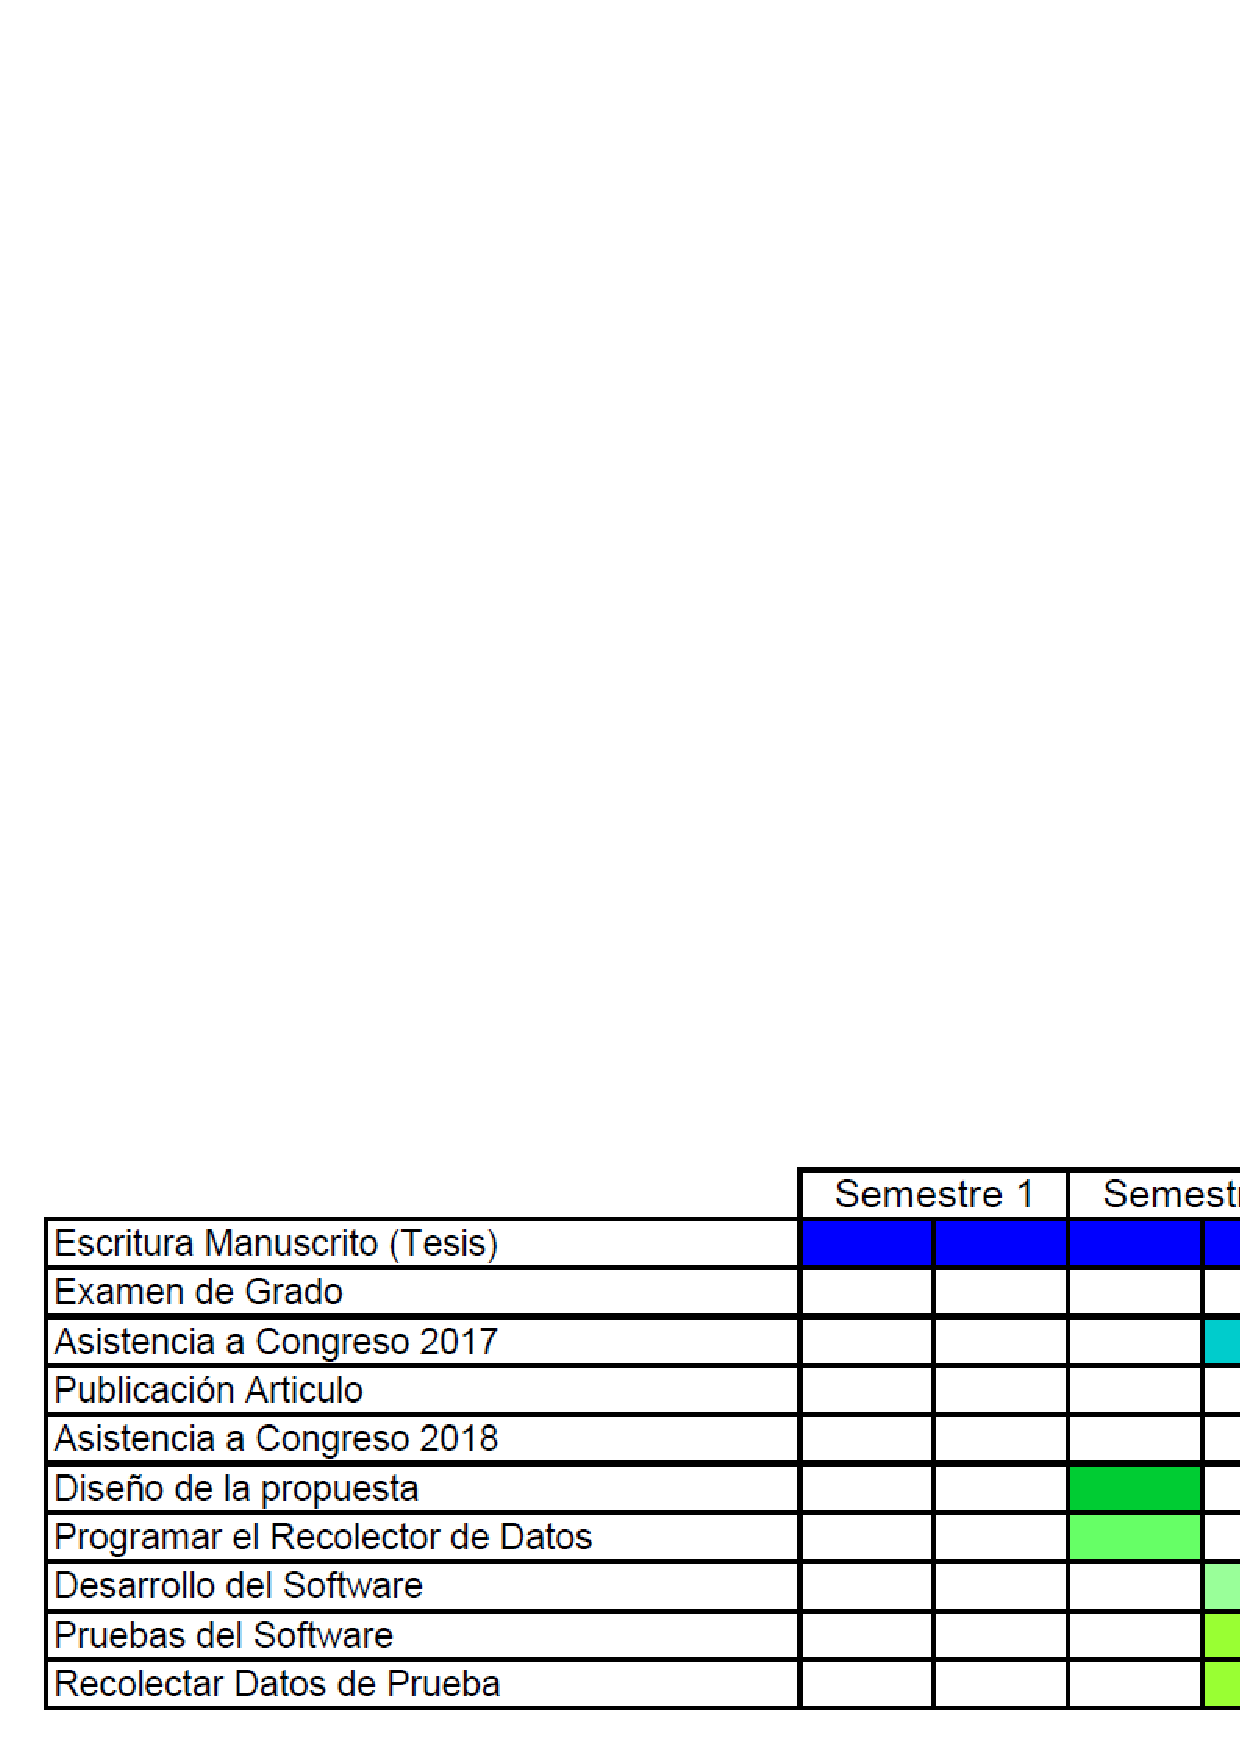
\includegraphics[width=1.0\columnwidth]{./CapituloI/Imagenes/Cronograma.PNG}
\caption{Gráfica de GANTT del cronograma de actividades.}
\end{figure} 
% Este documento se realizó con el propósito de proporcionale a los estudiantes del CIDETEC un machote en latex de la tesis. Espero que les sirva de ayuda.
% Atte: Dr. Miguel Gabriel Villarreal Cervantes.
%*********************************************************************************************************
%*********************************************************************************************************
% Capítulo I
\chapter{Introducción \label{cap1}}

La demanda de sistemas electromecánicos que proporcionen un alto
desempeño ...
$y=0$ y=0

Contenido \ref{FigLogo}...
\begin{figure}[h]
    \centering
  % Requires \usepackage{graphicx}
  
\includegraphics[scale=0.5]{CapituloI/Imagenes/logo_ipn.eps}\\
  \caption{Diagrama ...}\label{FigLogo}
\end{figure}

El capítulo \ref{cap1}...

En \cite{RolandSiegwart+IllanNourbakhsh},


Por lo tanto en este trabajo de investigación se propone, como un problema ....

\section{Planteamiento del problema}
Con base en lo mencionado previamente, en este trabajo de investigación se desarrollará ...


\section{Objetivos}
\begin{itemize}
  \item Establecer ...
  \item Desarrollar ...
  \item Validar ...
\end{itemize}

\section{Justificación}



\section{Metodología}
Con el propósito de desarrollar y lograr los objetivos propuestos en el presente trabajo de investigación, se plantearon siguientes metas:
\section*{Metas}
\begin{itemize}
  \item[I] Obtención y validación ...
  \item[II] Formulación ...
  \item[III] Establecimiento ...
  \item[IV] Implementación ...
  \item[V] Desarrollo ...
  \item[VI] Manufactura ...
  \item[VII] Validación numérica y experimental ...
  \item[VIII] Evaluación cuantitativa de los resultados ...
\end{itemize}





\section{Cronograma de actividades}



\begin{table}[h]
\centering
%EndExpansion
%

\begin{tabular}{|c|c|c|c|c|c|}
\hline
\multicolumn{6}{|c|}{Periodo 2013/02}\tabularnewline
\hline
\hline
Metas & Ago & Sep & Oct & Nov & Dic\tabularnewline
\hline
I & X & X & X & X & X\tabularnewline
\hline
II & X & X & X & X & \tabularnewline
\hline


\end{tabular}

\caption{Cronograma de Actividades I}
\label{reglasI}
\end{table}%
%EndExpansion



\begin{table}[h]
\centering
%EndExpansion
%

\begin{tabular}{|c|c|c|c|c|c|c|}
\hline
\multicolumn{7}{|c|}{Periodo 2014/01}\tabularnewline
\hline
\hline
Metas & Ene & Feb & Mar & Abr & May & Jun\tabularnewline
\hline
I & X & X & X & X & X & X\tabularnewline
\hline
III &  & X &  &  &  & \tabularnewline
\hline
IV.I & X & X & X & X & X & X\tabularnewline
\hline
V & X & X & X &  &  & \tabularnewline
\hline
VI &  & X & X &  &  & \tabularnewline
\hline


\end{tabular}
%

\caption{Conograma de Actividades II}
\label{reglasII}
\end{table}%



\begin{table}[h]
\centering
%EndExpansion
%

\begin{tabular}{|c|c|c|c|c|c|}
\hline
\multicolumn{6}{|c|}{Periodo 2014/02}\tabularnewline
\hline
\hline
Metas & Ago & Sep & Oct & Nov & Dic\tabularnewline
\hline
I & X & X &  &  & \tabularnewline
\hline
IV.II & X & X & X & X & X\tabularnewline
\hline
VII &  &  & X & X & \tabularnewline
\hline
VIII &  &  &  & X & X \tabularnewline
\hline
IX & X &  &  &  & \tabularnewline
\hline
X & X & X & X & X & X\tabularnewline
\hline
XV &  &  & X & X & X\tabularnewline
\hline
\end{tabular}
%

\caption{Conograma de Actividades III}
\label{reglasIII}
\end{table}%




\begin{table}[h]
\centering
%EndExpansion
%

\begin{tabular}{|c|c|c|c|c|c|c|}
\hline
\multicolumn{7}{|c|}{Periodo 2015/01}\tabularnewline
\hline
\hline
Metas & Ene & Feb & Mar & Abr & May & Jun\tabularnewline
\hline
I & X & X &  &  &  & \tabularnewline
\hline
XI & X & X & X & X &  & \tabularnewline
\hline
XII &  & X & X & X & X & \tabularnewline
\hline
XIII &  &  & X & X & X & \tabularnewline
\hline
XIV &  &  &  &  &  & X\tabularnewline
\hline
XV & X & X & X &  &  & \tabularnewline
\hline
\end{tabular}
%

\caption{Conograma de Actividades IV}
\label{reglasIV}
\end{table}% 




	

%%=========================================
\chapter{ Avances Recientes  \label{cap2}}
%=========================================


Las Opciones de accesibilidad de Microsoft Windows han permitido que su
 sistema operativo sea posible usarlo sin importar las condiciones físicas del
 usuario \cite{DanielHubbell2016},A continuación, se menciona una breve 
 descripción de estas opciones.

\begin{itemize}
	\item Lupa: Aumenta el tamaño del contenido de la pantalla para que sea más
	 fácil leerlo \cite{xatakaaccesiblilidad}.
	\item Narrador:  Esta función es una ayuda auditiva que ayuda a saber cuáles
	 son las ventanas abiertas y su contenido, por medio de una voz sintetizada
	 \cite{xatakaaccesiblilidad}.
	\item Teclado en pantalla: Como su nombre lo indica es un teclado virtual
	 con el cual podemos escribir presionando la pantalla, en caso de ser un
	 dispositivo táctil, o presionando los botones con el ratón
	 \cite{xatakaaccesiblilidad}.
	 \item Contraste alto: Otra ayuda visual para poder distinguir mejor los
	  elementos en pantalla modificando el contraste de Windows
	  \cite{xatakaaccesiblilidad}.
	  \item Reconocimiento de voz: Es una herramienta de dictado con la cual se
	   puede escribir y manipular aplicaciones e incluso el mismo sistema
	   operativo por medio de comandos de voz \cite{support14213}.
\end{itemize}
	   
Aunque no esta considerado dentro de las opciones de accesibilidad de Windows,
 el asistente Cortana facilita la realización de algunas tareas por medio de
 comandos de voz, por ejemplo, apertura de programas, la manipulación de
 recordatorios, mensajes de texto y correo electrónico \cite{support17214}. 

Los archivos por lotes (Batch o Script Shell) \cite{Silberschatz1999} son
 archivos que contienen instrucciones para el sistema operativo en formato
 ASCII por lo que son dependientes de él, por lo general tienen la extensión
 .bat o .sh, sin embargo, para el caso de UNIX esto no es obligatorio. En la
 imagen~\ref{fig:script} se muestra el código de un archivo por lotes y la 
 ejecucion en consola.


\begin{figure}[H]
\centering
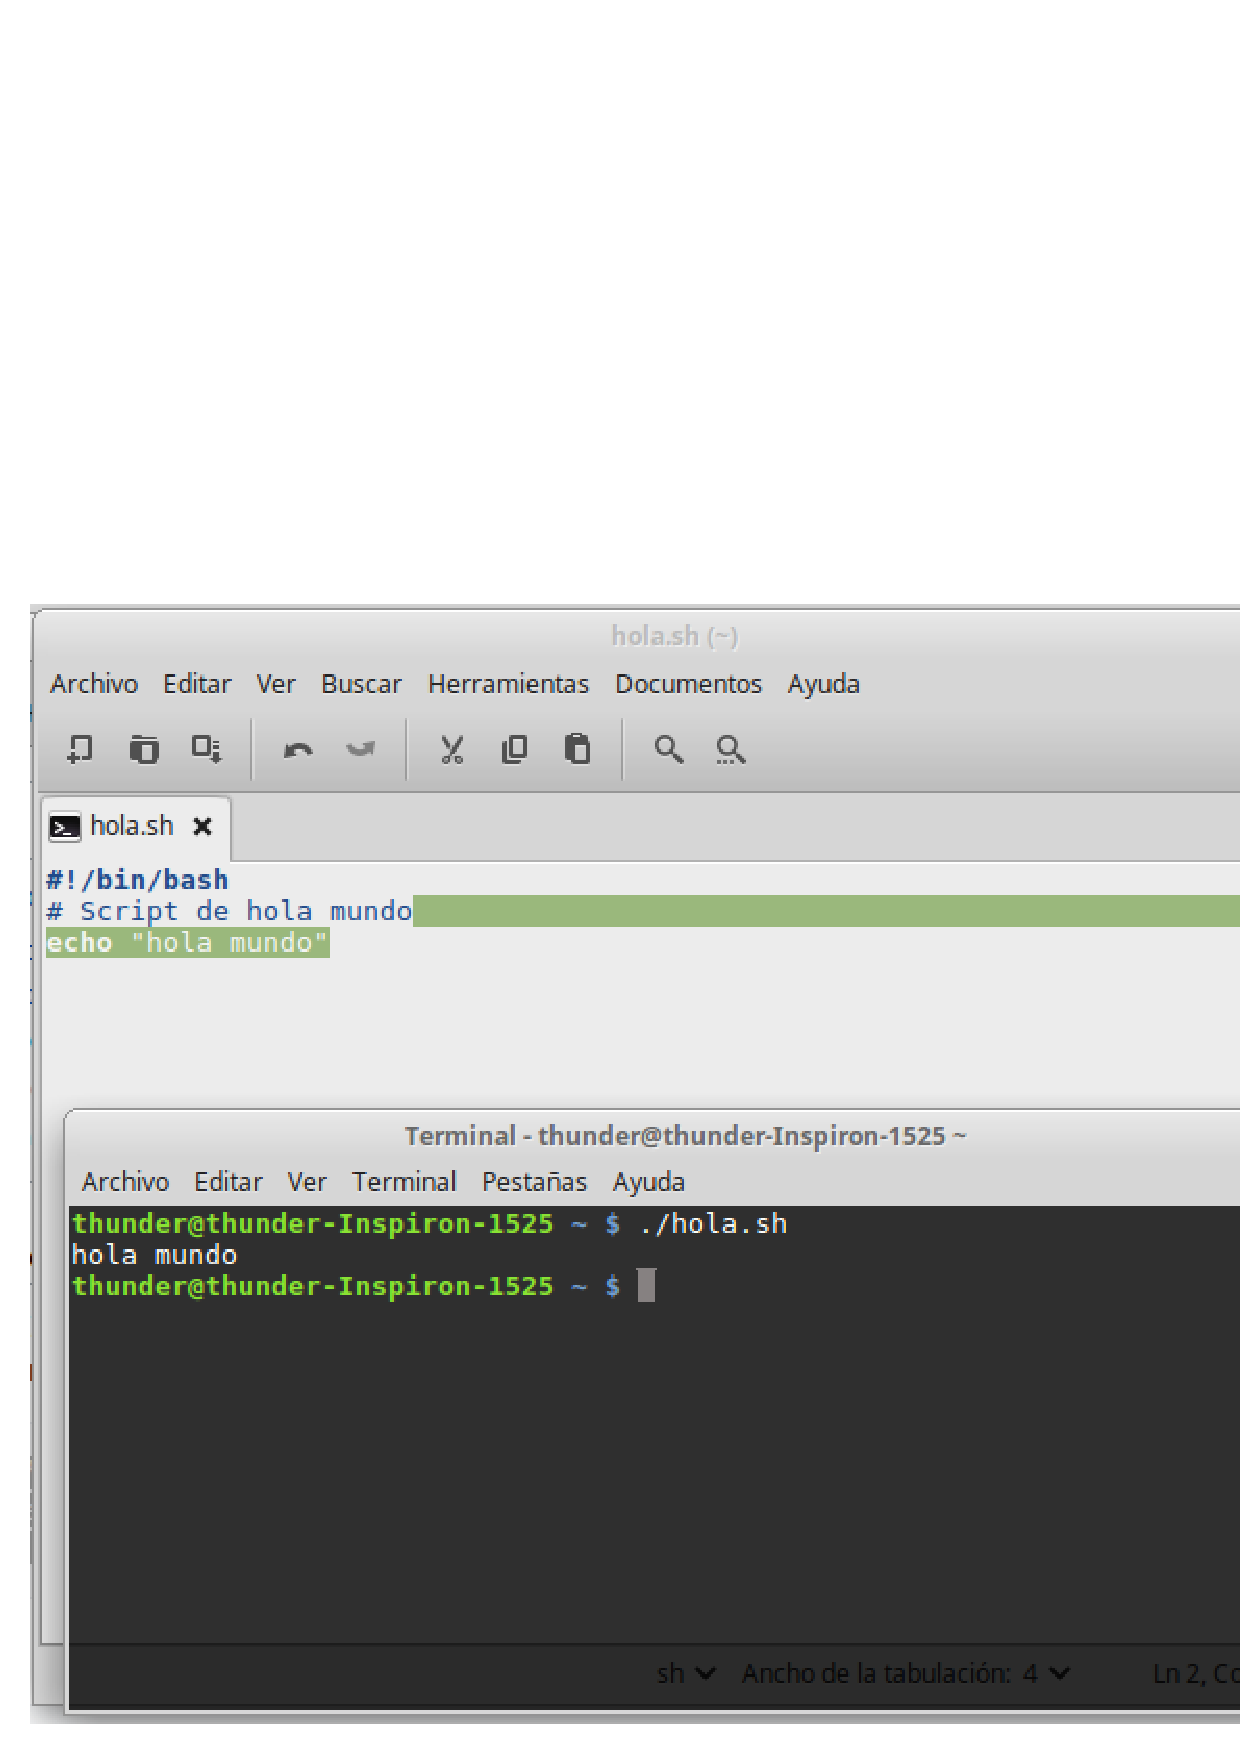
\includegraphics[width=0.7\columnwidth]{CapituloI/Imagenes/Script.png}
\caption{Ejecución de un archivo por lotes en Linux.}
\label{fig:script}
\end{figure}


Pulover's Macro Creator\cite{Batista}, desarrollado y mantenido
 principalmente por Rodolfo U. Batista, es una herramienta de automatización
 y creación de scripts basada en el lenguaje ``AutoHotKey''. Este creador de
 macros facilita la tarea de la creación del script por medio de su interfaz
 gráfica ó con la grabadora de macros que proporciona. Entre sus
 características destaca el proporcionar control de ventanas en segundo plano
 y sentencias de control(ciclos y condicionales). En la imagen
 ~\ref{fig:macros} se puede observar la interfaz de usuario del software.


\begin{figure}[H]
\centering
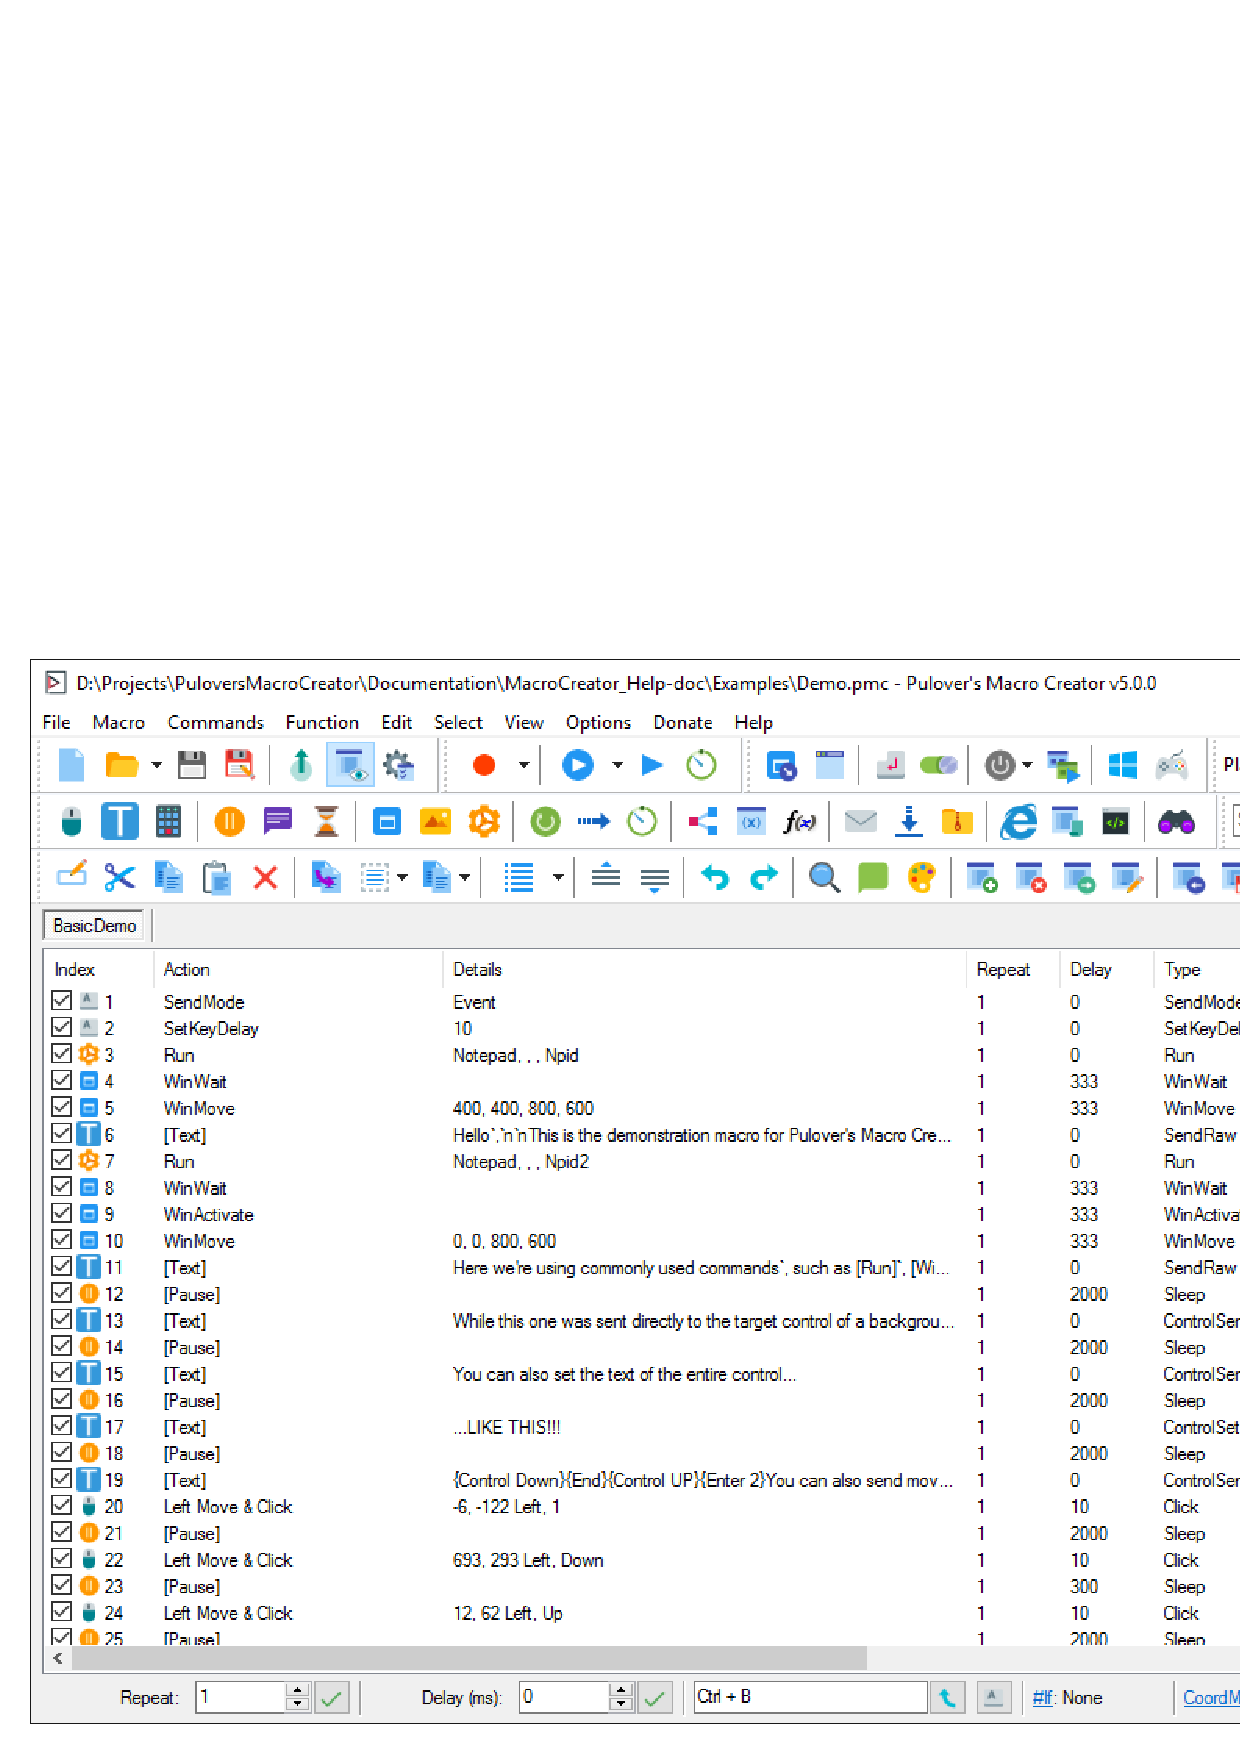
\includegraphics[width=0.7\columnwidth]{CapituloI/Imagenes/Macros.png}
\caption{Interfaz de usuario de Pulover's Macro Creator con una macro de
 ejemplo.}
\label{fig:macros}
\end{figure}



Un trabajo desarrollado por la Universidad de Tsukuba en
 Japón\cite{Nakano2006}, tiene por objetivo el crear un oponente virtual
 al nivel de un oponente humano que represente un reto para el jugador. Para
 lograr esto se crearon perfiles con las estrategias de los jugadores y
 posteriormente se reproducen en otra partida, en la imagen~\ref{fig:imitat}
 se muestra el entorno del juego.


\begin{figure}[H]
\centering
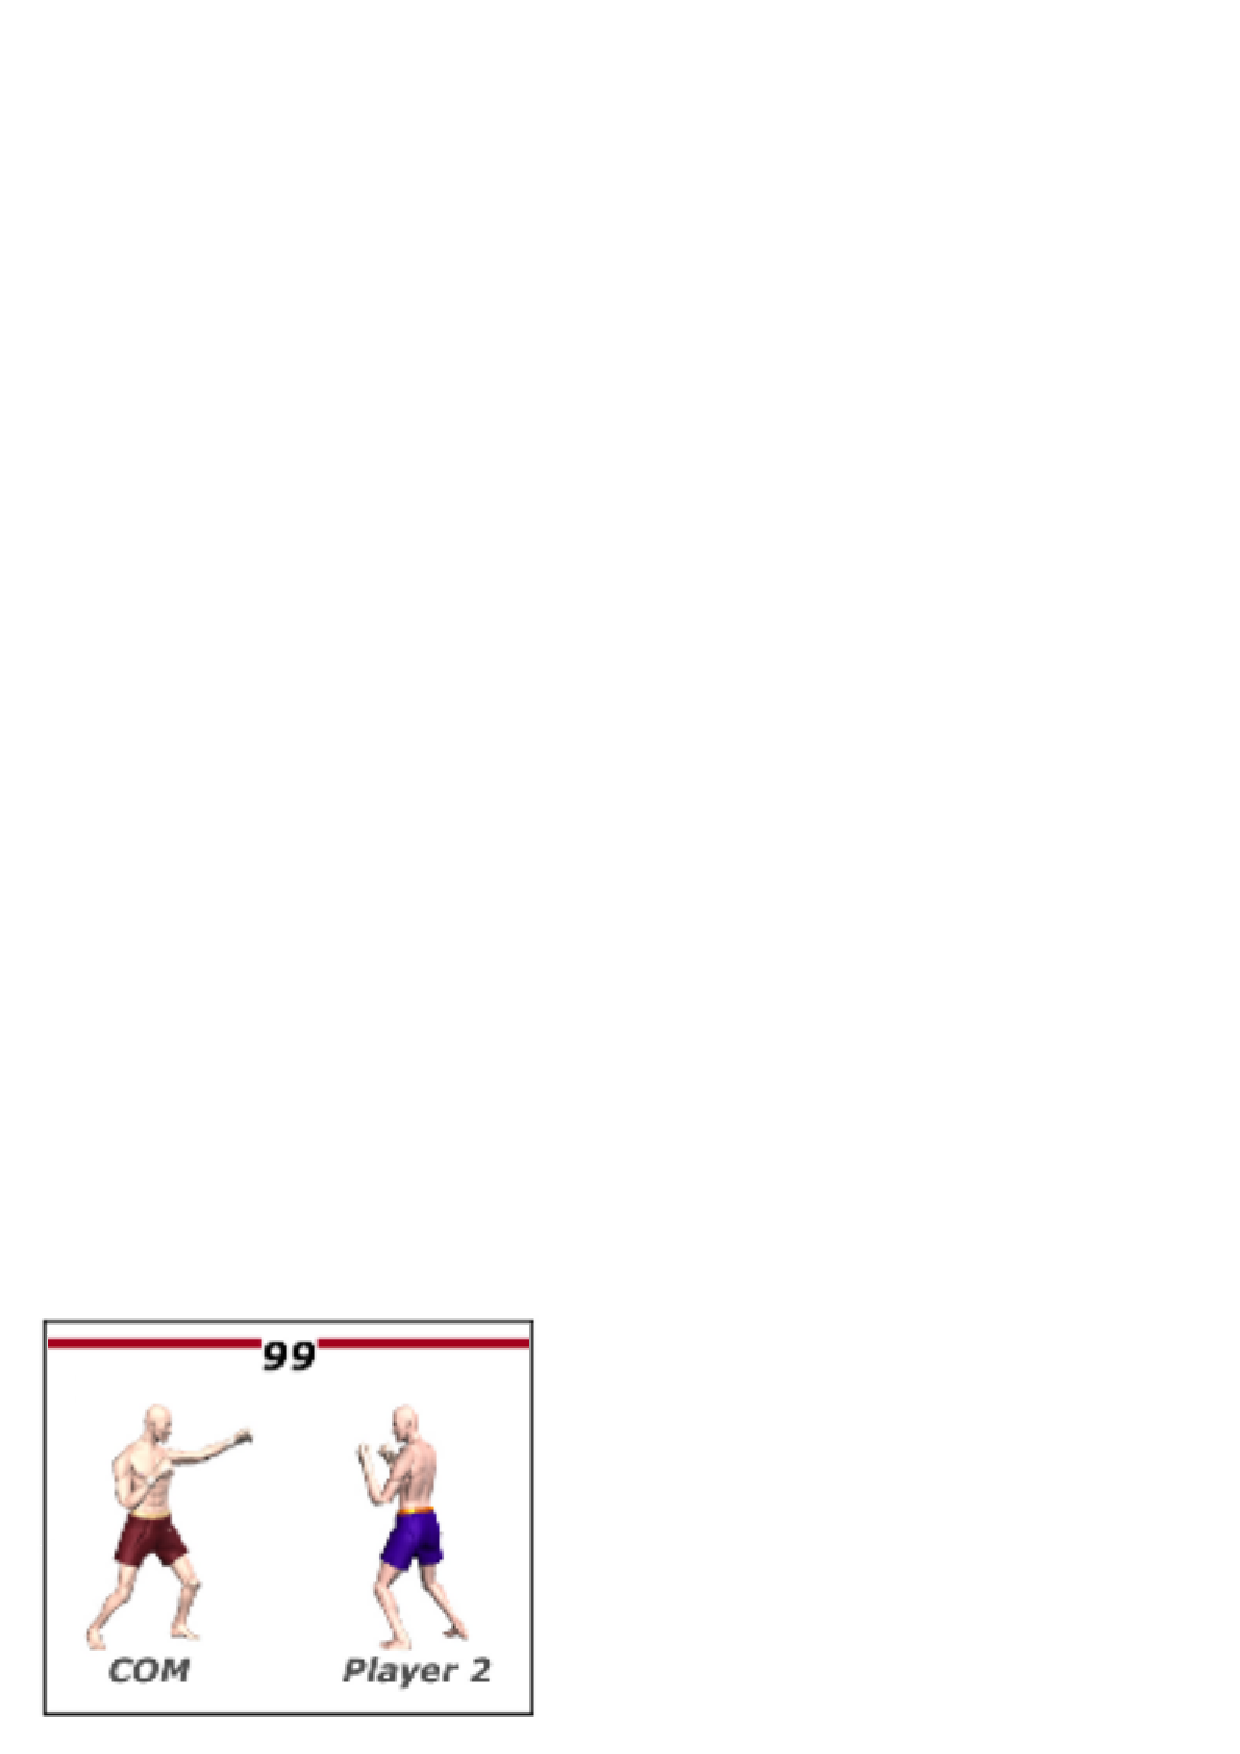
\includegraphics[width=0.5\columnwidth]{CapituloI/Imagenes/Imitating.png}
\caption{Ambiente del juego de acción.}
\label{fig:imitat}
\end{figure}


En el trabajo desarrollado en la Universidad Tecnológica de Lanzhou en China
 \cite{Zhang2017},hacen un análisis del comportamiento del soldador experto
 humano utilizando un sistema de inferencia neurodifuso adaptativo (ANFIS,
 por sus siglas en inglés) para su automatización, considerando las variables
 de los materiales usados y caracterizando la tarea del soldador humano.
 En la imagen~\ref{fig:syswelding} se puede apreciar el sistema experimental
  resultante del proyecto mencionado.


\begin{figure}[H]
\centering
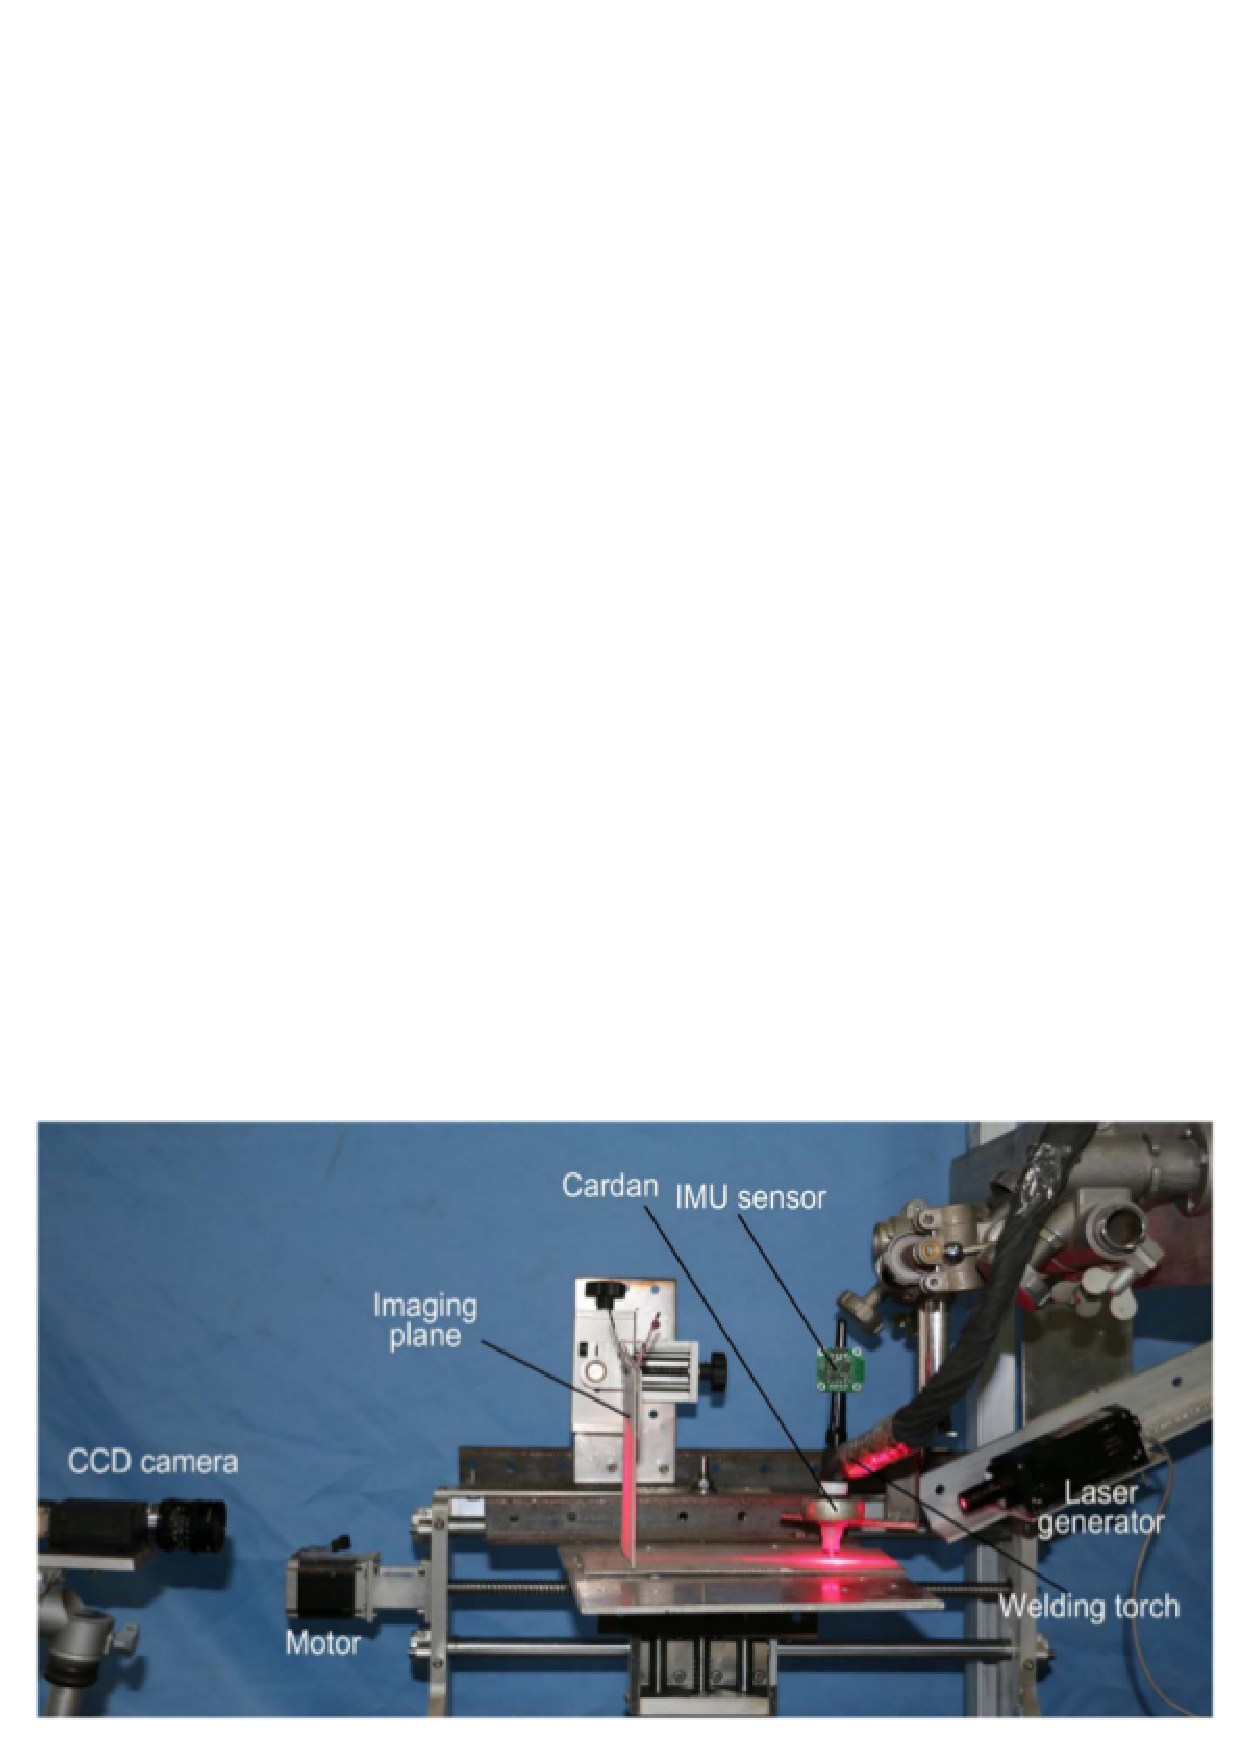
\includegraphics[width=0.8\columnwidth]{CapituloI/Imagenes/Welding.png}
\caption{Sistema experimental de la soldadora.}
\label{fig:syswelding}
\end{figure} 
 

En el ambiente artístico \cite{Nishiguchi2017}, el trabajo desarrollado en
 Japón por la Universidad de artes de Tokyo y la Universidad de Osaka, cuyo
 objetivo era brindar un comportamiento natural humano a un Robot Humanoide.
 Para cumplir esto utilizaron el conocimiento del director de escena Hirata,
 que dada la precisión en sus instrucciones a los actores, facilita la
 traducción de esas órdenes a las reglas para el robot humanoide, además,
 desarrollaron una interfaz de usuario para que el manejo del robot sea más
 sencillo, ayudando a los principiantes, ya que proporcionan menos datos se
 puede obtener buenos resultados. Como se puede observar en la imagen
 ~\ref{fig:theatricalrob} el robot llego a desempeñar un amigo del
 personaje principal en la obra ``Night on the milky way train''
 (El tren nocturno de la vía láctea) en un escenario real.


\begin{figure}[H]
\centering
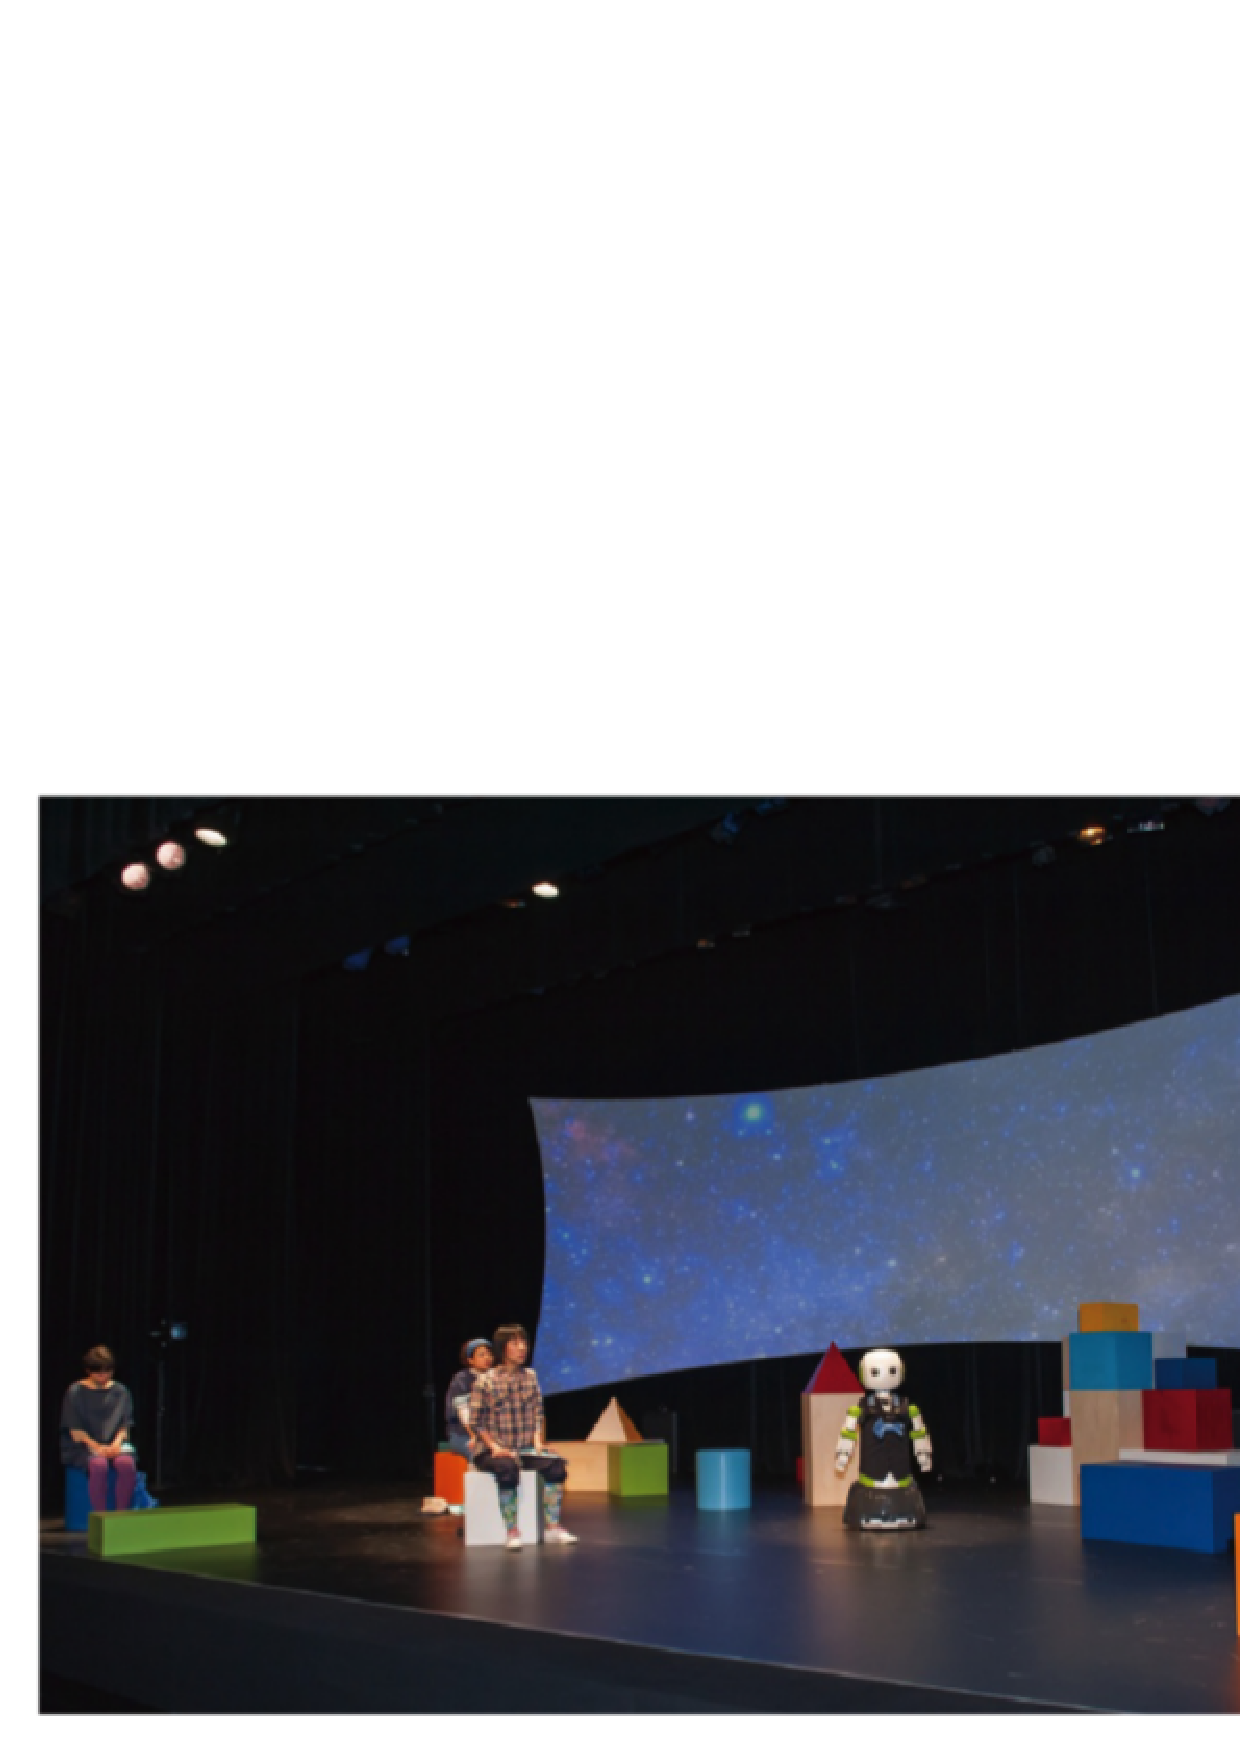
\includegraphics[width=0.8\columnwidth]{CapituloI/Imagenes/Theatrical.png}
\caption{Robot humanoide actor en escenario real.}
\label{fig:theatricalrob}
\end{figure} 


El trabajo desarrollado por la Universidad de Plymouth, Universidad de
 Lincoln ambas en el Reino Unido y la Universidad de Gante en Bélgica
 \cite{Senft2016}, realiza un análisis comparativo de su método SPARC (Supervised
 Progressively Autonomous Robot Competencies) con el IRL (Interactive
 Reinforcement Learning), estos dos métodos se basan en el aprendizaje 
 automático de un robot, haciendo que un ser humano con conocimiento del tema
 apruebe la actividad que está realizando o que va a realizar el robot.
 Ambos sistemas fueron probados en un ambiente virtual nombrado ``sophie’s
 kitchen''(La cocina de Sofia) cuyo objetivo es hornear un pastel, 
 la imagen ~\ref{fig:sparcrob} muestra al robot en la cocina con los materiales
 necesarios para realizar la tarea. 
 
\begin{figure}[H]
\centering
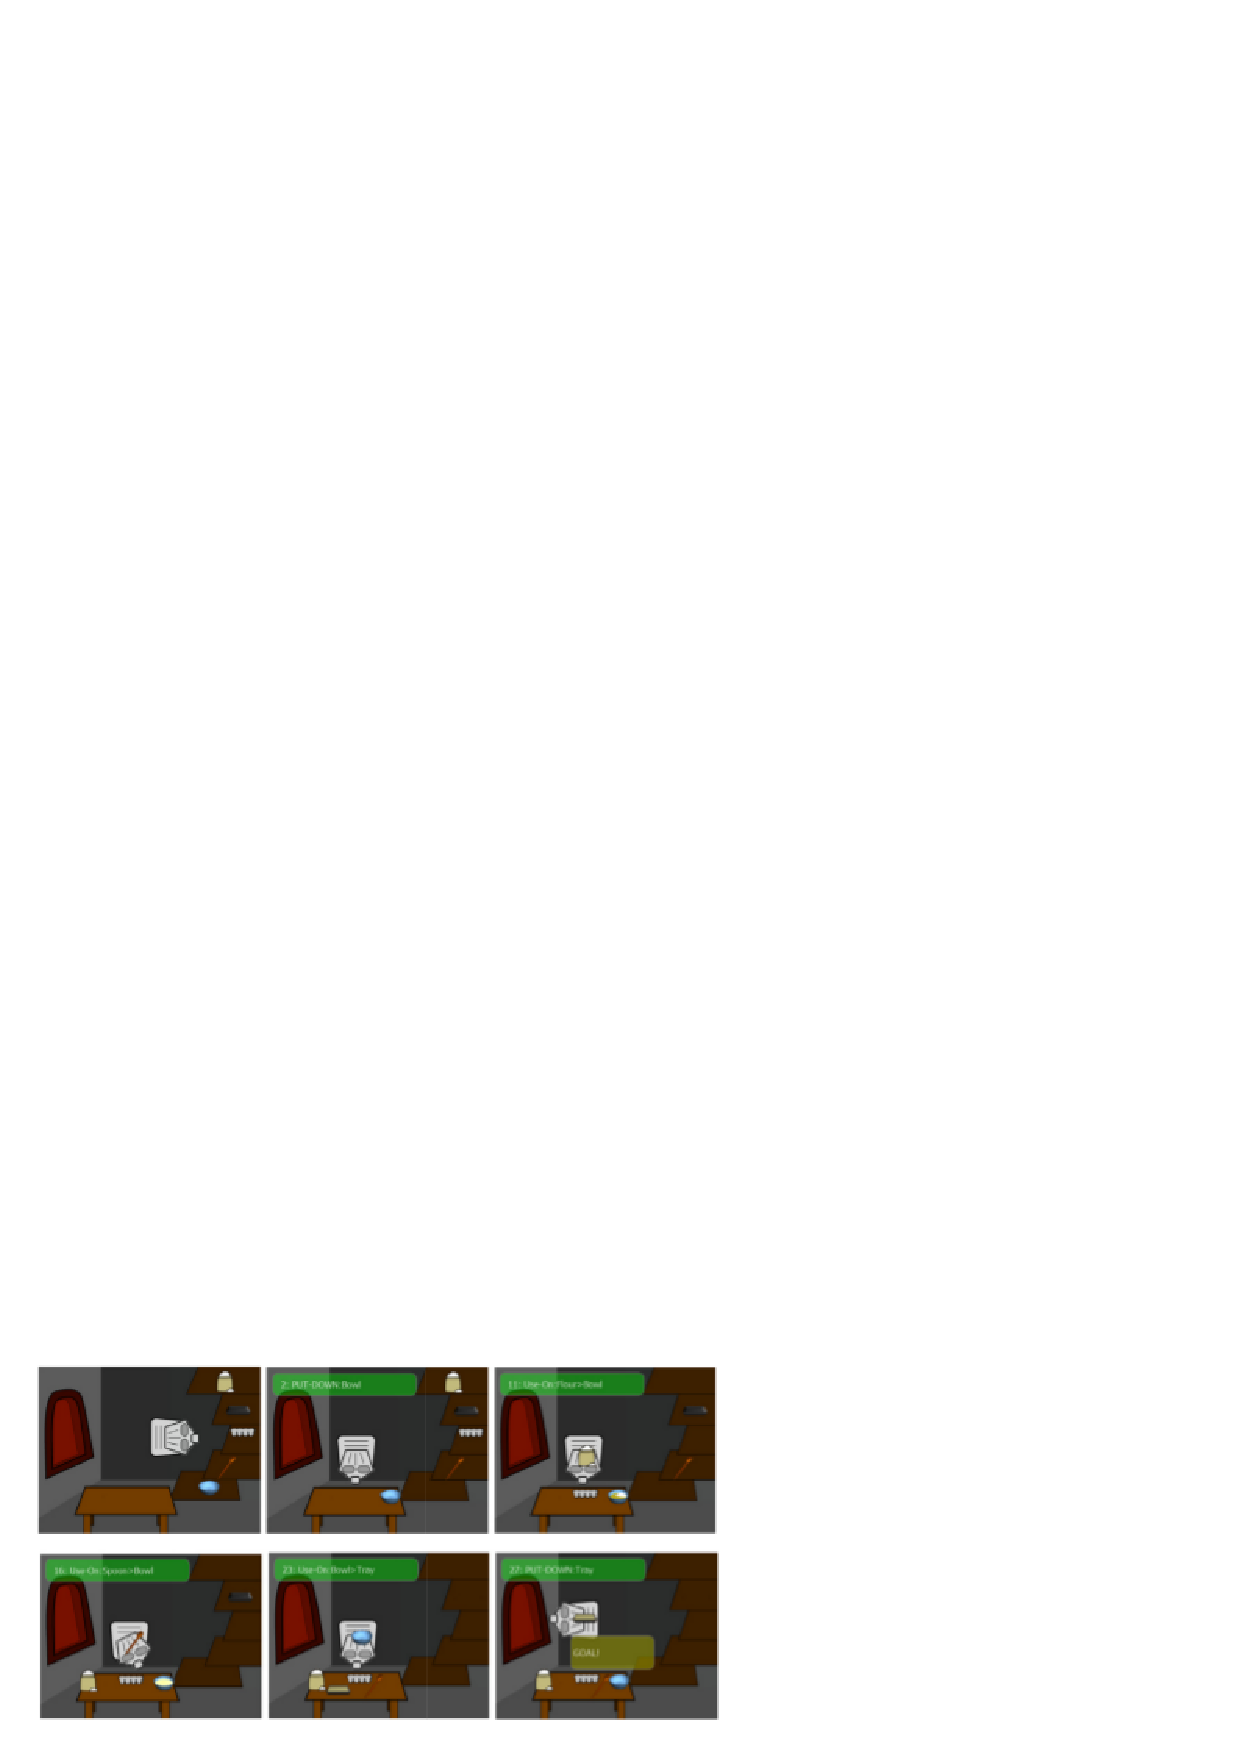
\includegraphics[width=0.8\columnwidth]{CapituloI/Imagenes/Sparc.png}
\caption{Robot virtual en “sophie’s kitchen”(La cocina de Sofia).}
\label{fig:sparcrob}
\end{figure}


El trabajo realizado en la Universidad Nacional Chiao Tung y el Instituto
 Politécnico Kaohsiung ambos en Taiwán\cite{Chang1996}, propone un algoritmo
 que imite el comportamiento del aprendizaje humano como una solución al
 aprendizaje automático en ambientes imperfectos, por ejemplo, cuando la
 información esta incompleta. Este algoritmo demuestra en los experimentos
 realizados ser superior al algoritmo ID3 y PRISM.
 %Para la tesis

%%=========================================
\chapter{Marco Teórico \label{cap3}}
%=========================================

\section{Teoría de árboles}
En términos matemáticos un árbol es un grafo $T$ el cual se puede definir de
 la siguiente forma\cite{SUSANNAS.EPP2012}:

\begin{itemize}
	\item ``Un grafo se llama árbol si y solo si, está libre de circuitos y
	 es conexo.''
	\item ``Un vértice de grado 1 en $T$ se denomina un vértice terminal (o
	 una hoja).''
	\item ``Un vértice de grado superior a 1 en $T$ es un vértice interno (o
	 un vértice de rama).''
\end{itemize}

Los arboles son muy usados en la actualidad ya que permiten  darle sentido a
 la información contenida, gracias a la asociatividad, parentización y
 prioridad que este permite de manera implícita. Entre sus usos múltiples en
 el área de la informática se pueden destacar los  siguientes; relaciones
 entre módulos de programación, arboles de decisión en inteligencia artificial
 y representaciones gramáticas\cite{gutierrez1999estructuras}.  

Una forma de ver a un árbol puede ser como un solo nodo, esté recibe el nombre
 de  nodo raíz, al cual se le puede enraizar un sinfín de arboles lo que da
 origen  a un árbol con otras características, dependiendo del resultado se le
 puede clasificar en alguno de los modelos existentes, por ejemplo; árbol 
 general o árbol binario\cite{gutierrez1999estructuras}. 

El árbol general es un modelo con una cantidad indeterminada de nodos hijos,
 mientras que el árbol binario es un caso particular del árbol general ya que
 este tiene la característica de tener siempre en cada nodo 2 nodos hijos como
 máximo, cabe mencionar que este es uno de los modelos a mas usados, así como
 el ultimo caso mencionado, hay arboles que tienen una cantidad fija de nodos
 hijos, de manera general estos son llamados arboles n-arios
 \cite{gutierrez1999estructuras}. %Para la tesis

%%==================================================================================
\chapter{Capitulo XXX}
\label{cap4}
%\setcounter{secnumdepth}{5}
%==================================================================================
 %Para la tesis

%\include{CapituloV/CapituloV} %Para la tesis

%%=========================================
\chapter{Conclusiones y perspectivas \label{cap6}}
%=========================================

\cite{RolandSiegwart+IllanNourbakhsh} %Para la tesis

%\backmatter
%*********************************************************************************************************
%*********************************************************************************************************
% Bibliografía
\bibliographystyle{unsrt}
\bibliography{bibliografia/Bibliografia}

%\addcontentsline{toc}{chapter}{Bibliografía}
%\begin{thebibliography}{X}
%
%	\bibitem{RolandSiegwart+IllanNourbakhsh}
%	\textsc{Roland Siegwart, Illan R. Nourbakhsh.},
%	\textit{``Introduction to Autonomous Mobile Robots''},
%	Massachusetts Institute of Technology, 2004
%
%	\bibitem{villarreal-Alvarez:16}
%	\textsc{M. G. Villarreal-Cervantes and J. Alvarez-Gallegos},
%	\textsc{"Off-line PID control tuning for a planar parallel robot using DE variants, Expert Systems with Applications"},
%	Expert Systems with Applications. 2016.
%
%\end{thebibliography} %Para la propuesta y la tesis

%%*********************************************************************************************************
%*********************************************************************************************************
% Apéndices
\appendix

\chapter{Apendice XXX \label{Apen:A}}



\chapter{Publicaciones \label{ApenD}}
A continuación se presenta una lista de los artículos publicados en congresos de arbitraje nacional que se realizaron durante el periodo en que se realizo la tesis de maestría


 %Para la tesis

%\include{Apendice/Apendice/ApendiceC/ApendiceC}
\end{document}